%%%%%%%%%%%%%%%%%%%%%%%%%%%%%%%%%%%%%%
%%  
%% Chapter 2: OpenMP overview
%%
%%%%%%%%%%%%%%%%%%%%%%%%%%%%%%%%%%%%%%

\def\ArtDir{02.Overview/figures}%



\chapter[OpenMP overview]{OpenMP overview}
\label{chapter:OMPoverview}

Compared to other parallel programming languages in use today, OpenMP is old.  
The first release (OpenMP 1.0 for Fortran) was in 1997.  
It started as the simplest way we could think of for applications programmers  
in high performance computing to write multithreaded code.  The focus
was on parallelizing loops and the full OpenMP definition took only 40 pages.

At the time we are writing this book, OpenMP is at release 5.1.  The specification covers
Fortran, C and C++.  It includes multiple ways to parallelize loops, create explicit tasks, 
 vectorize loops, manage complex memory hierarchies, and much 
more (including programming GPUs, of course).

With OpenMP 1.0, the entire language could be covered in a single day of study.  Now, it takes months if
not years to master the entire specification.  New versions of the specification come out roughly every 
two years.  Hence, once the language is mastered, something new comes along to expand its scope 
even future.

The situation with OpenMP would be unbearably frustrating, if not for one simple fact.  Nobody
uses the entire language.  OpenMP programmers learn the foundational terminology of OpenMP and 
a simplified common core of the language elements of OpenMP.  Most of the time, that common core
is all a programmer needs.  When additional features of OpenMP are needed, programmers look them up in 
the specification.  By learning and then using just those parts of OpenMP needed to solve a programming 
problem, the complexity of OpenMP is manageable and that inner-simplicity that motivated us at the beginning
shines through.

In this chapter, we will cover those core elements of OpenMP that all programmers use.   We will be brief
and expose them through an investigation of the three fundamental design patterns of multithreaded programming
with OpenMP; loop-level parallelism, SPMD, and Task-parallelism.   Then we will go back through the core
elements of OpenMP and explain how they are organized around the behavior of both implied and explicit tasks.
This is essential since we can't explain GPU programming in OpenMP without using those details.  We 
then close the chapter with an overview of our journey into GPU programming with OpenMP.  

%------------------------------------------------------------------------------------------------------------------        
\section{OpenMP: foundational concepts}
\label{sec:OMPconcepts}

I will describe the fork-join model and the concept of thread teams.  

I need a fork-join figure

%Figure from common core book: 1 
\begin{figure}[!htbp]
%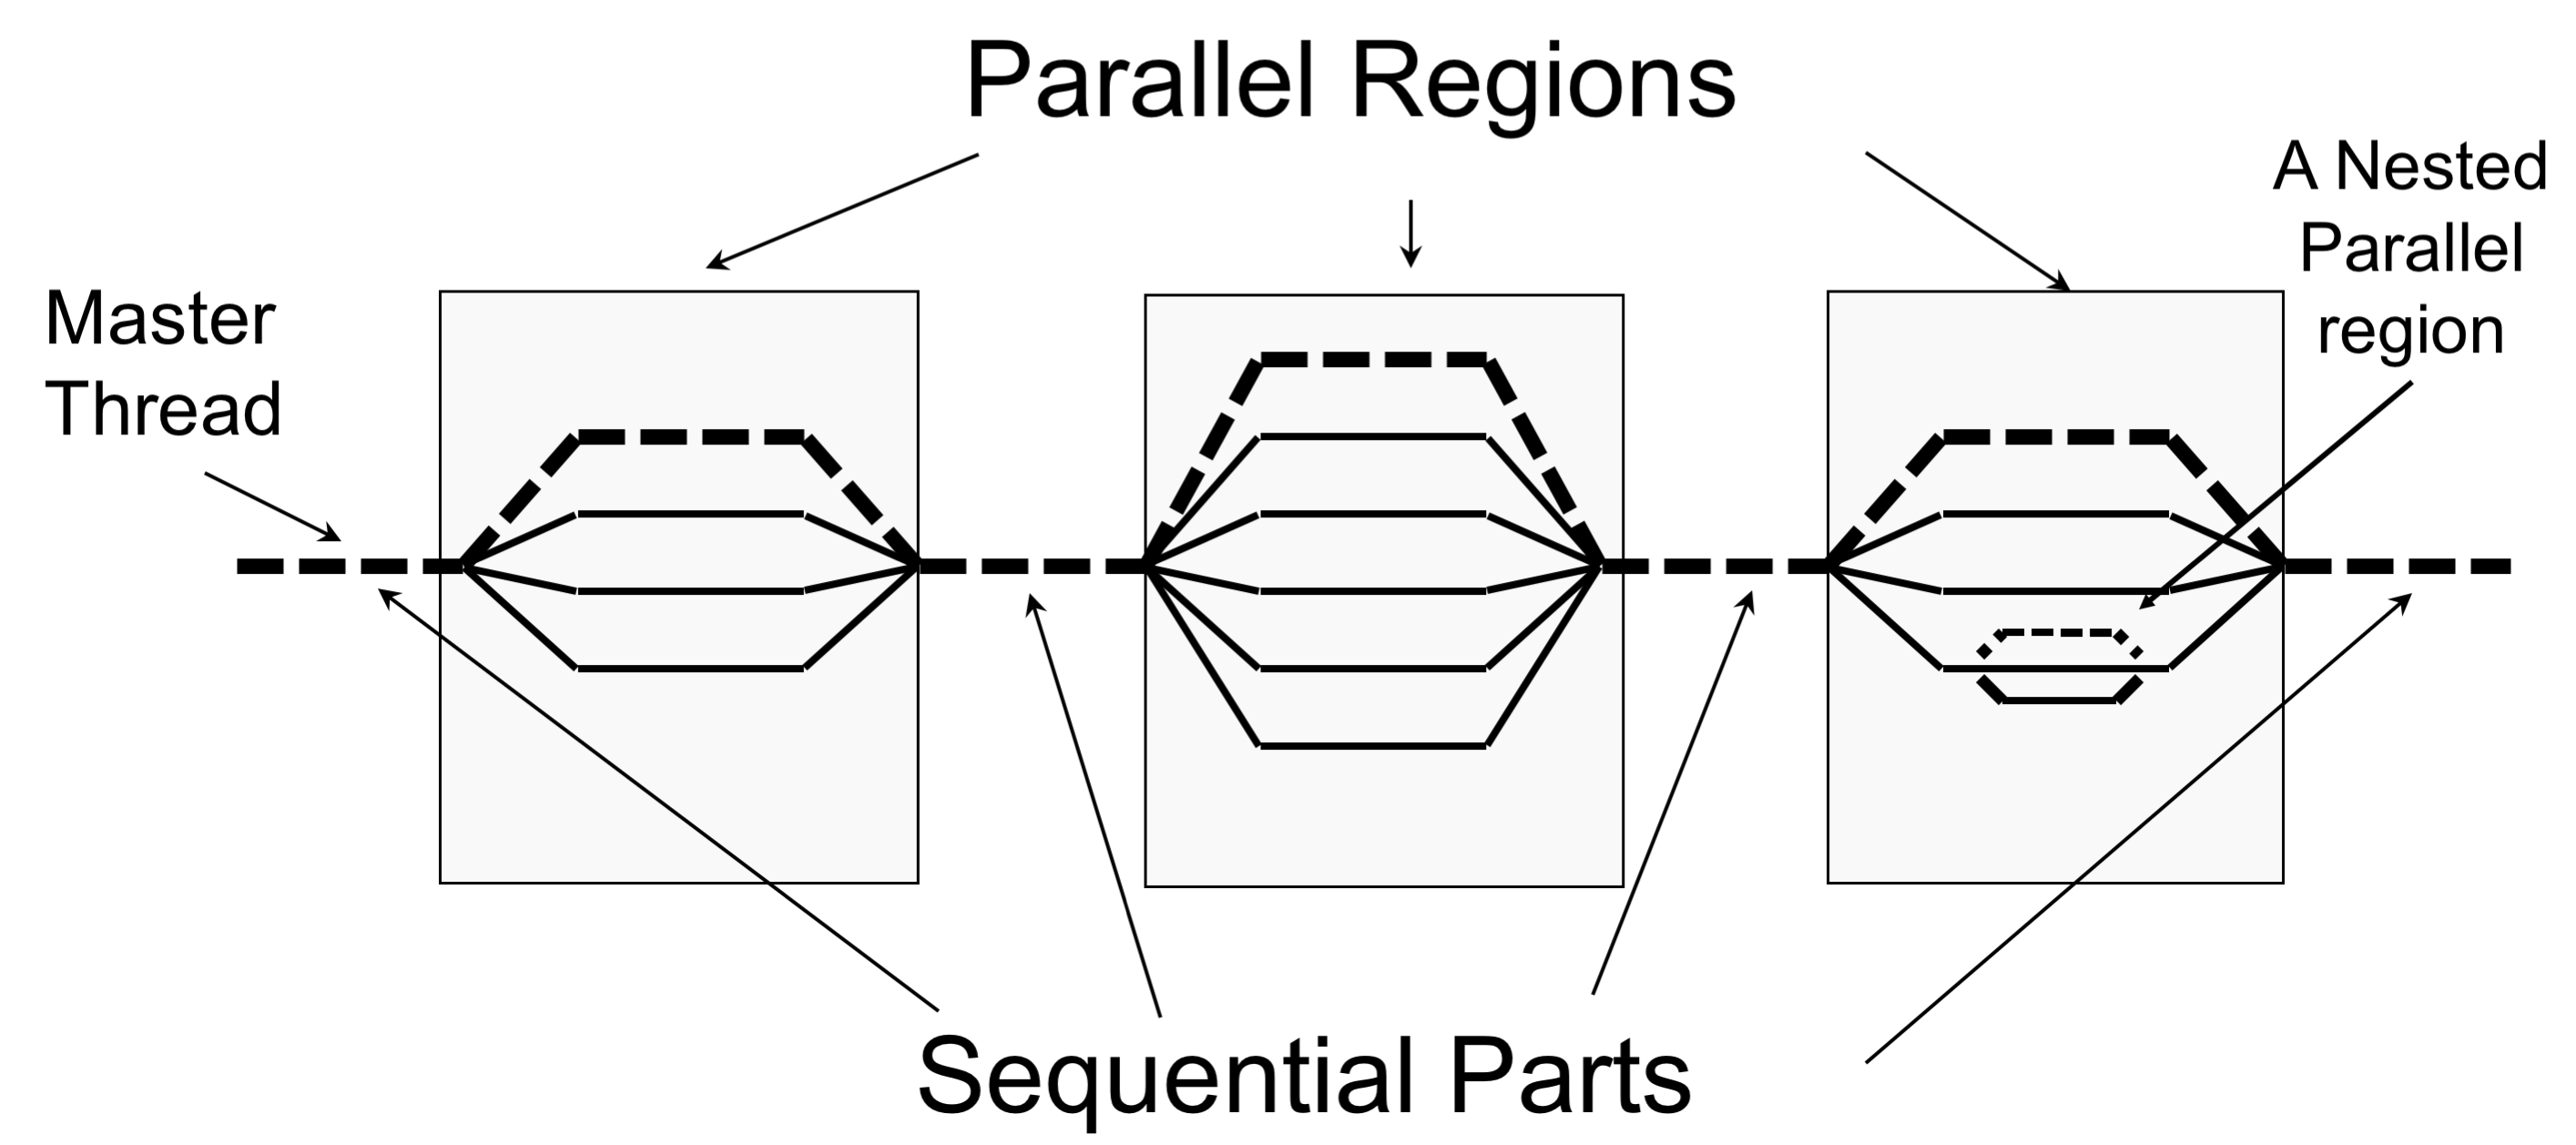
\includegraphics[width=\textwidth]{\ArtDir/ParallelRegions}
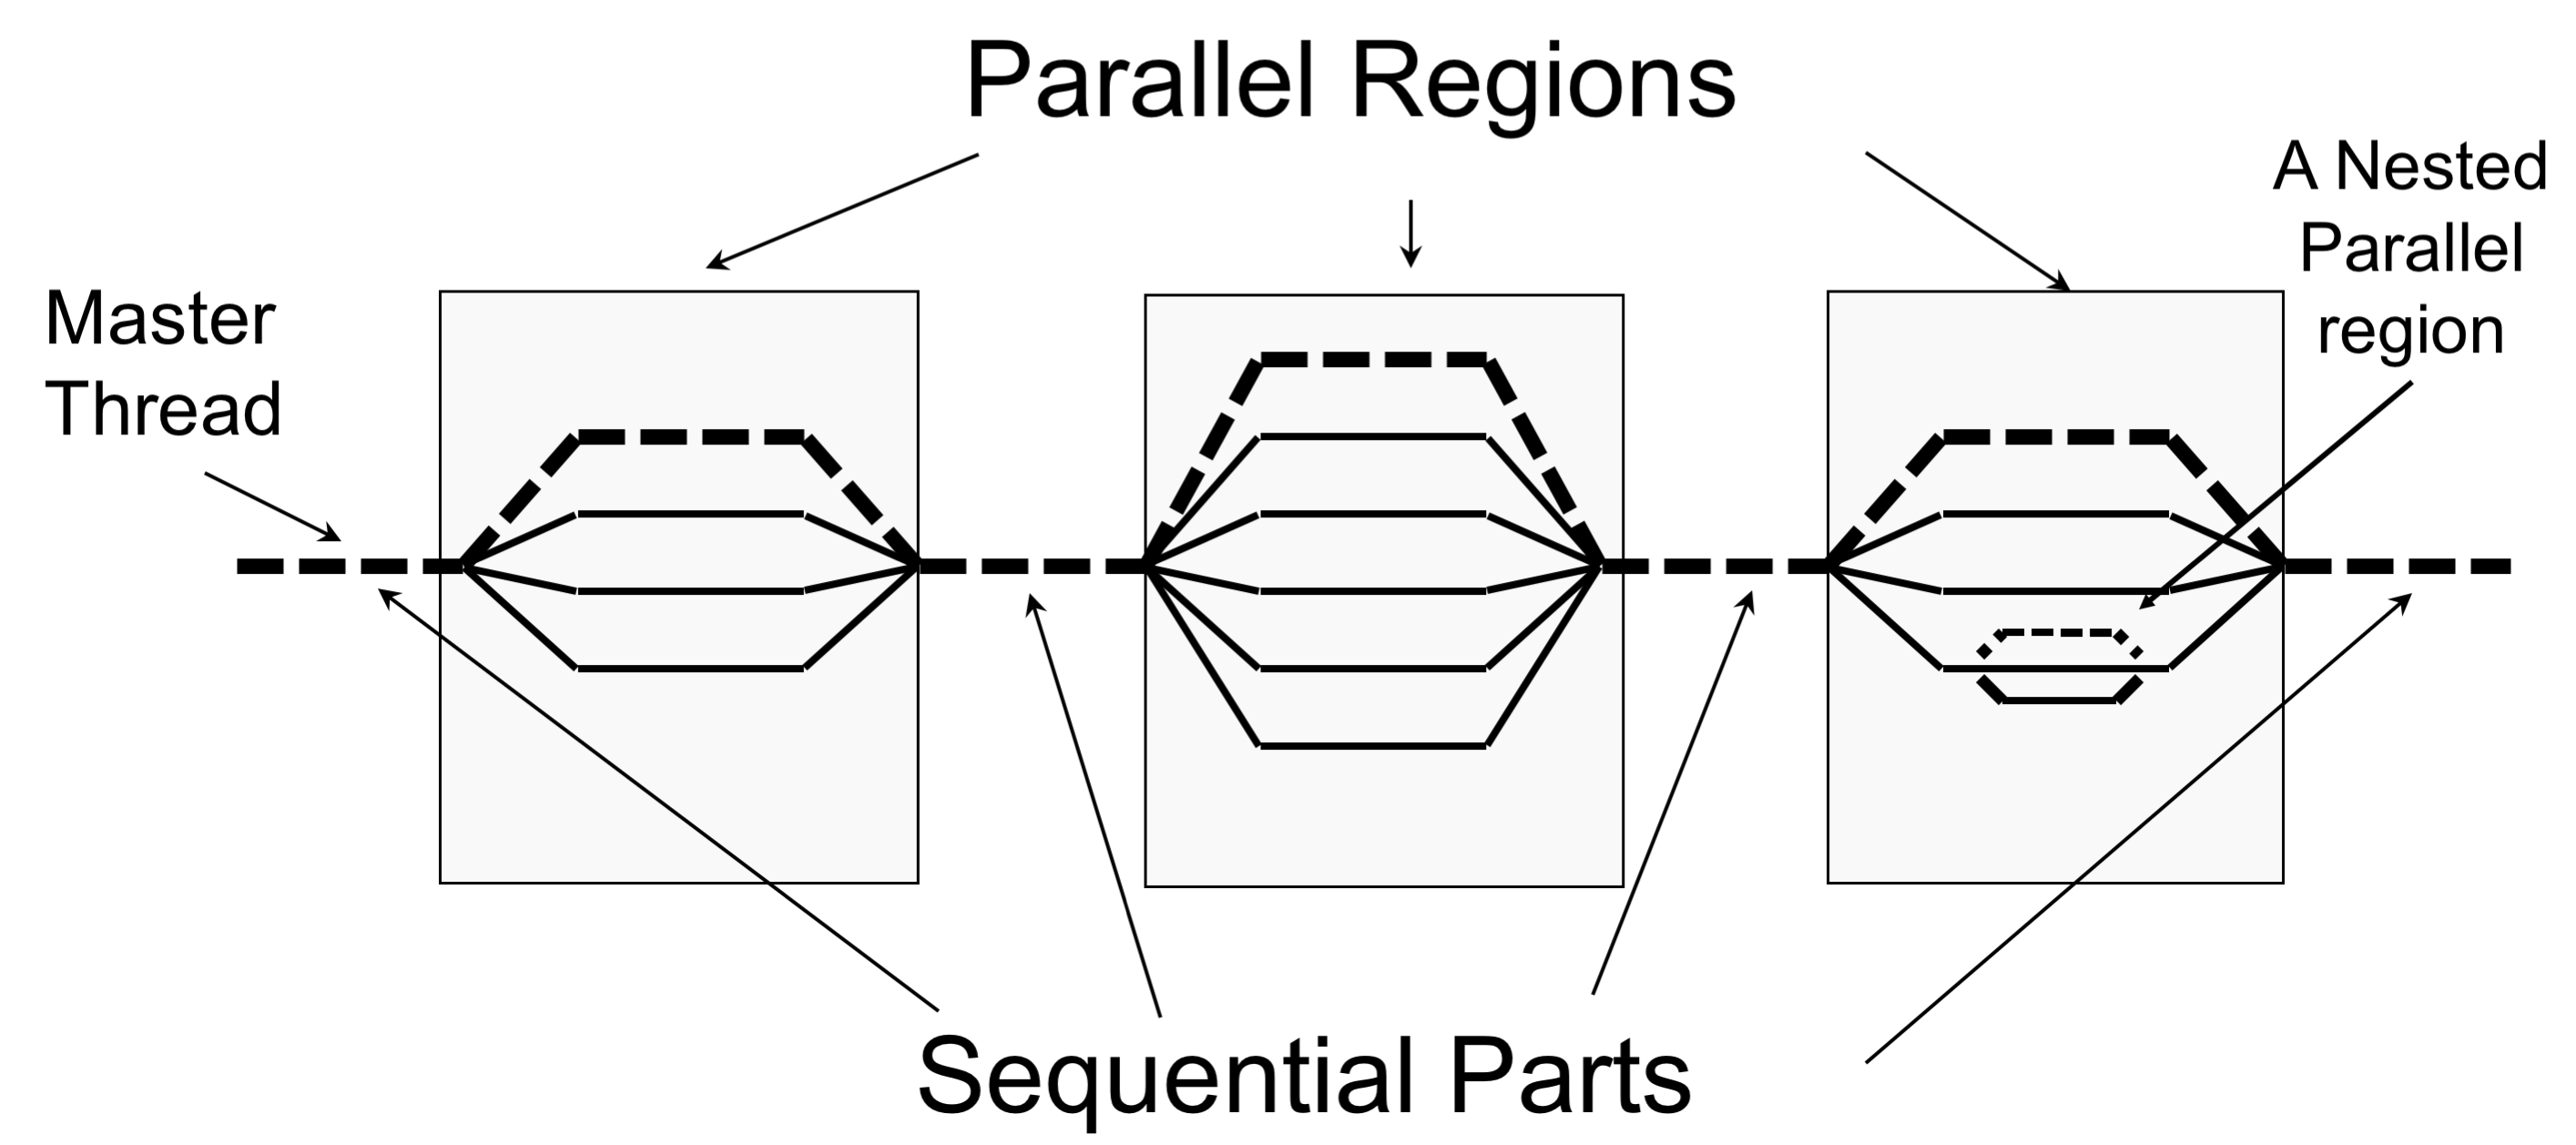
\includegraphics[width=4.2in]{\ArtDir/ParallelRegions}
\centering
\caption
{\textbf{The fork-join model} -- \small 
A program starts as a single thread. It creates (or \emph{forks})
a team of threads each of which executes a block of code.  When done, the threads
\emph{join} (i.e., are destroyed) and the single original thread continues. 
}
\label{fig:regions}
\end{figure}

%Figure from common core book: 1 




I need a code figure for structured blocks and examples of directive formats.

A figure for stack vs. heap.    The anatomy of a process and its relationship to threads.


\begin{itemize}
\item Directives, clauses, structured blocks, environment variables, library routines
\item a team of threads
\item Memory: stack vs heap
\item default rules of data sharing
\item The openMP data environment: concepts of private vs. shared. 
\end{itemize}




\begin{itemize}
  \item Parallel: threads in a team.
  \item Clauses to change effects: num\_threads, etc.
  \item Keep simple enough so reader knows notation, but refer to Common Core and Using OpenMP book for more details.
\end{itemize}



\begin{itemize}
  \item vector add.
  \item arrays allocated on the stack instead of heap.
  \item no reduction yet.
  \item can reuse this as the first target example without needing map clauses.
  \item stack arrays might also be useful for first target example to highlight data sharing clauses.
\end{itemize}




\begin{itemize}
  \item What is a relaxed shared memory model
  \item Synchronization and the need to order operations
  \item Need to be careful how we explain shared memory given the memory sharing rules between host/target we will introduce later.
\end{itemize}

%Text and table from common core book: 2
\begin{table}[!htbp]
\centering
\caption{\textbf{General form of directives in C/C++ and Fortran} -- \small  
The combination of a directive and a structured 
block is called a \emph{construct}.
}
\label{tab:directives}
\begin{tabular}{|l|}
\hline
\textbf{C/C++ directive format and an example with a structured block}  \\
\hline
                                           \\
\ompbcparallel \ompclauses  \\
                                           \\
\hline 
\ompbcparallel \texttt{  private(x)}    \\
\texttt{\{}                                                    \\
\texttt{  ... code executed by each thread}    \\
\texttt{\}}                                                \\
\\
\hline
\textbf{Fortran directive format and an example with a structured block}\\
\hline
                           \\
\ompbfparallel \ompclauses \\
\\
\hline
\ompbfparallel \texttt{  private(x)}    \\ 
\texttt{  ... code executed by each thread}  \\     
\ompbfparallelend \\
\hline
\end{tabular}
\end{table}

The basic syntax of directives in OpenMP is shown in Table~\ref{tab:directives}. C and C++ are block structured
languages.  The language definition includes the concept of a block where a block is one line of code or 
multiple lines of code between curly braces \{ and \}.  Hence, we can use the features of C and C++
to define the structured block associated with an OpenMP construct.  Fortran, however, is not
block structured. For Fortran, we need to add a directive to indicate the end of a block.  
As with C and C++, a 
block in Fortran is one statement or a set of statements between the opening directive and a 
directive that terminates the block (e.g., the  \code{!$omp end parallel} in 
Table~\ref{tab:directives}).
%end of: Text and table from common core book: 2



%Text and table from common core book: 3


\begin{figure}[!htbp]
%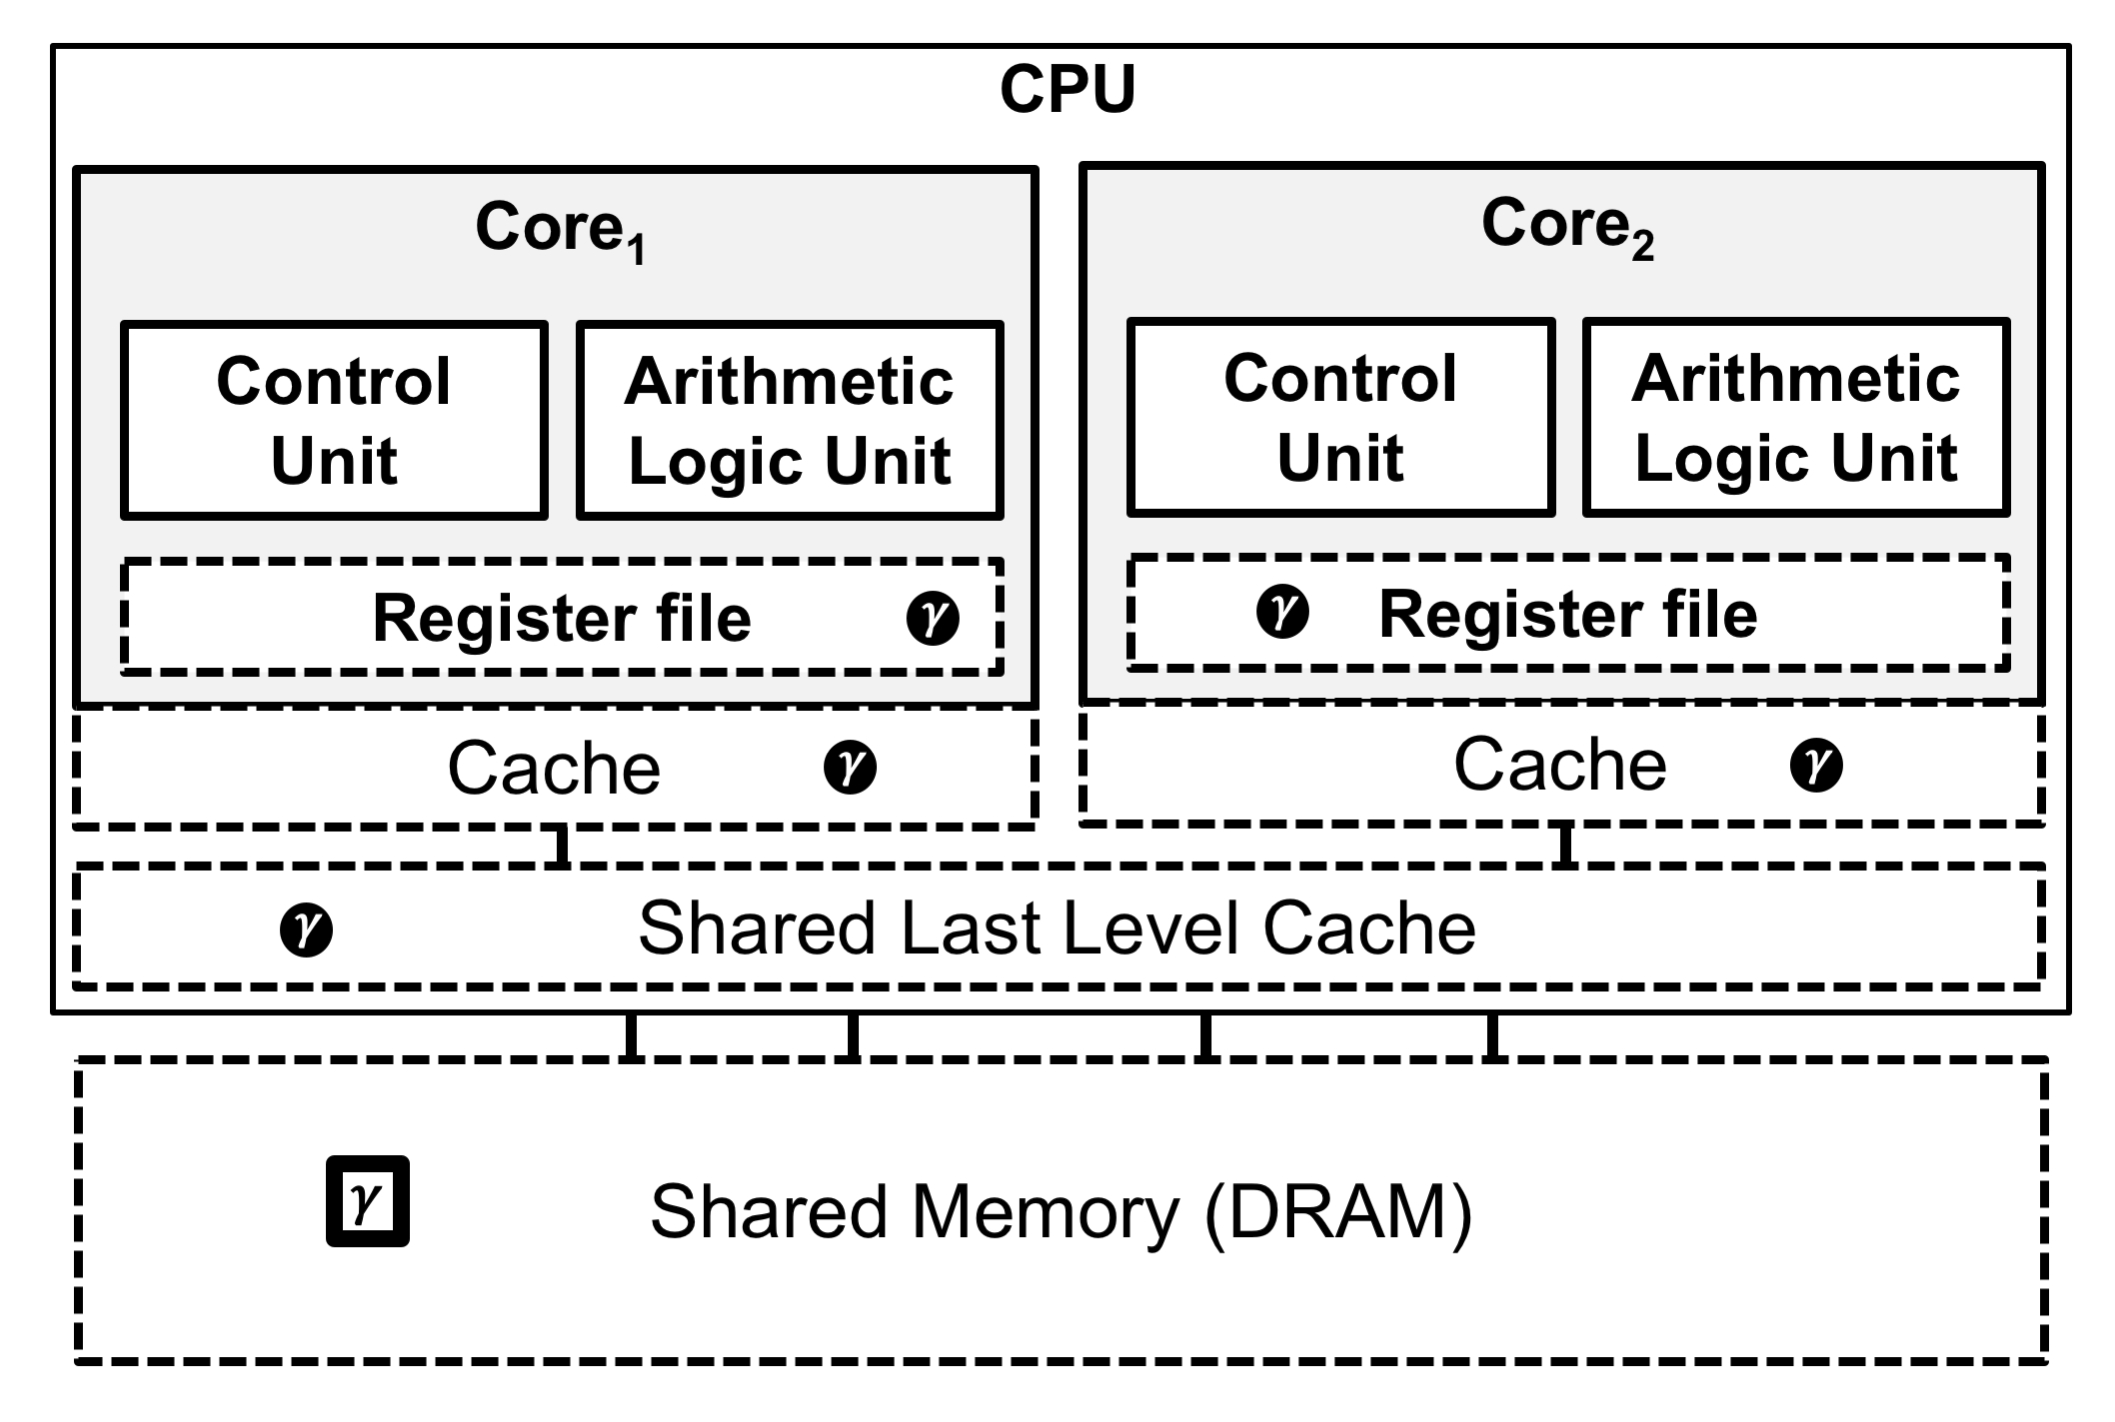
\includegraphics[width=\textwidth]{\ArtDir/MemoryModel}
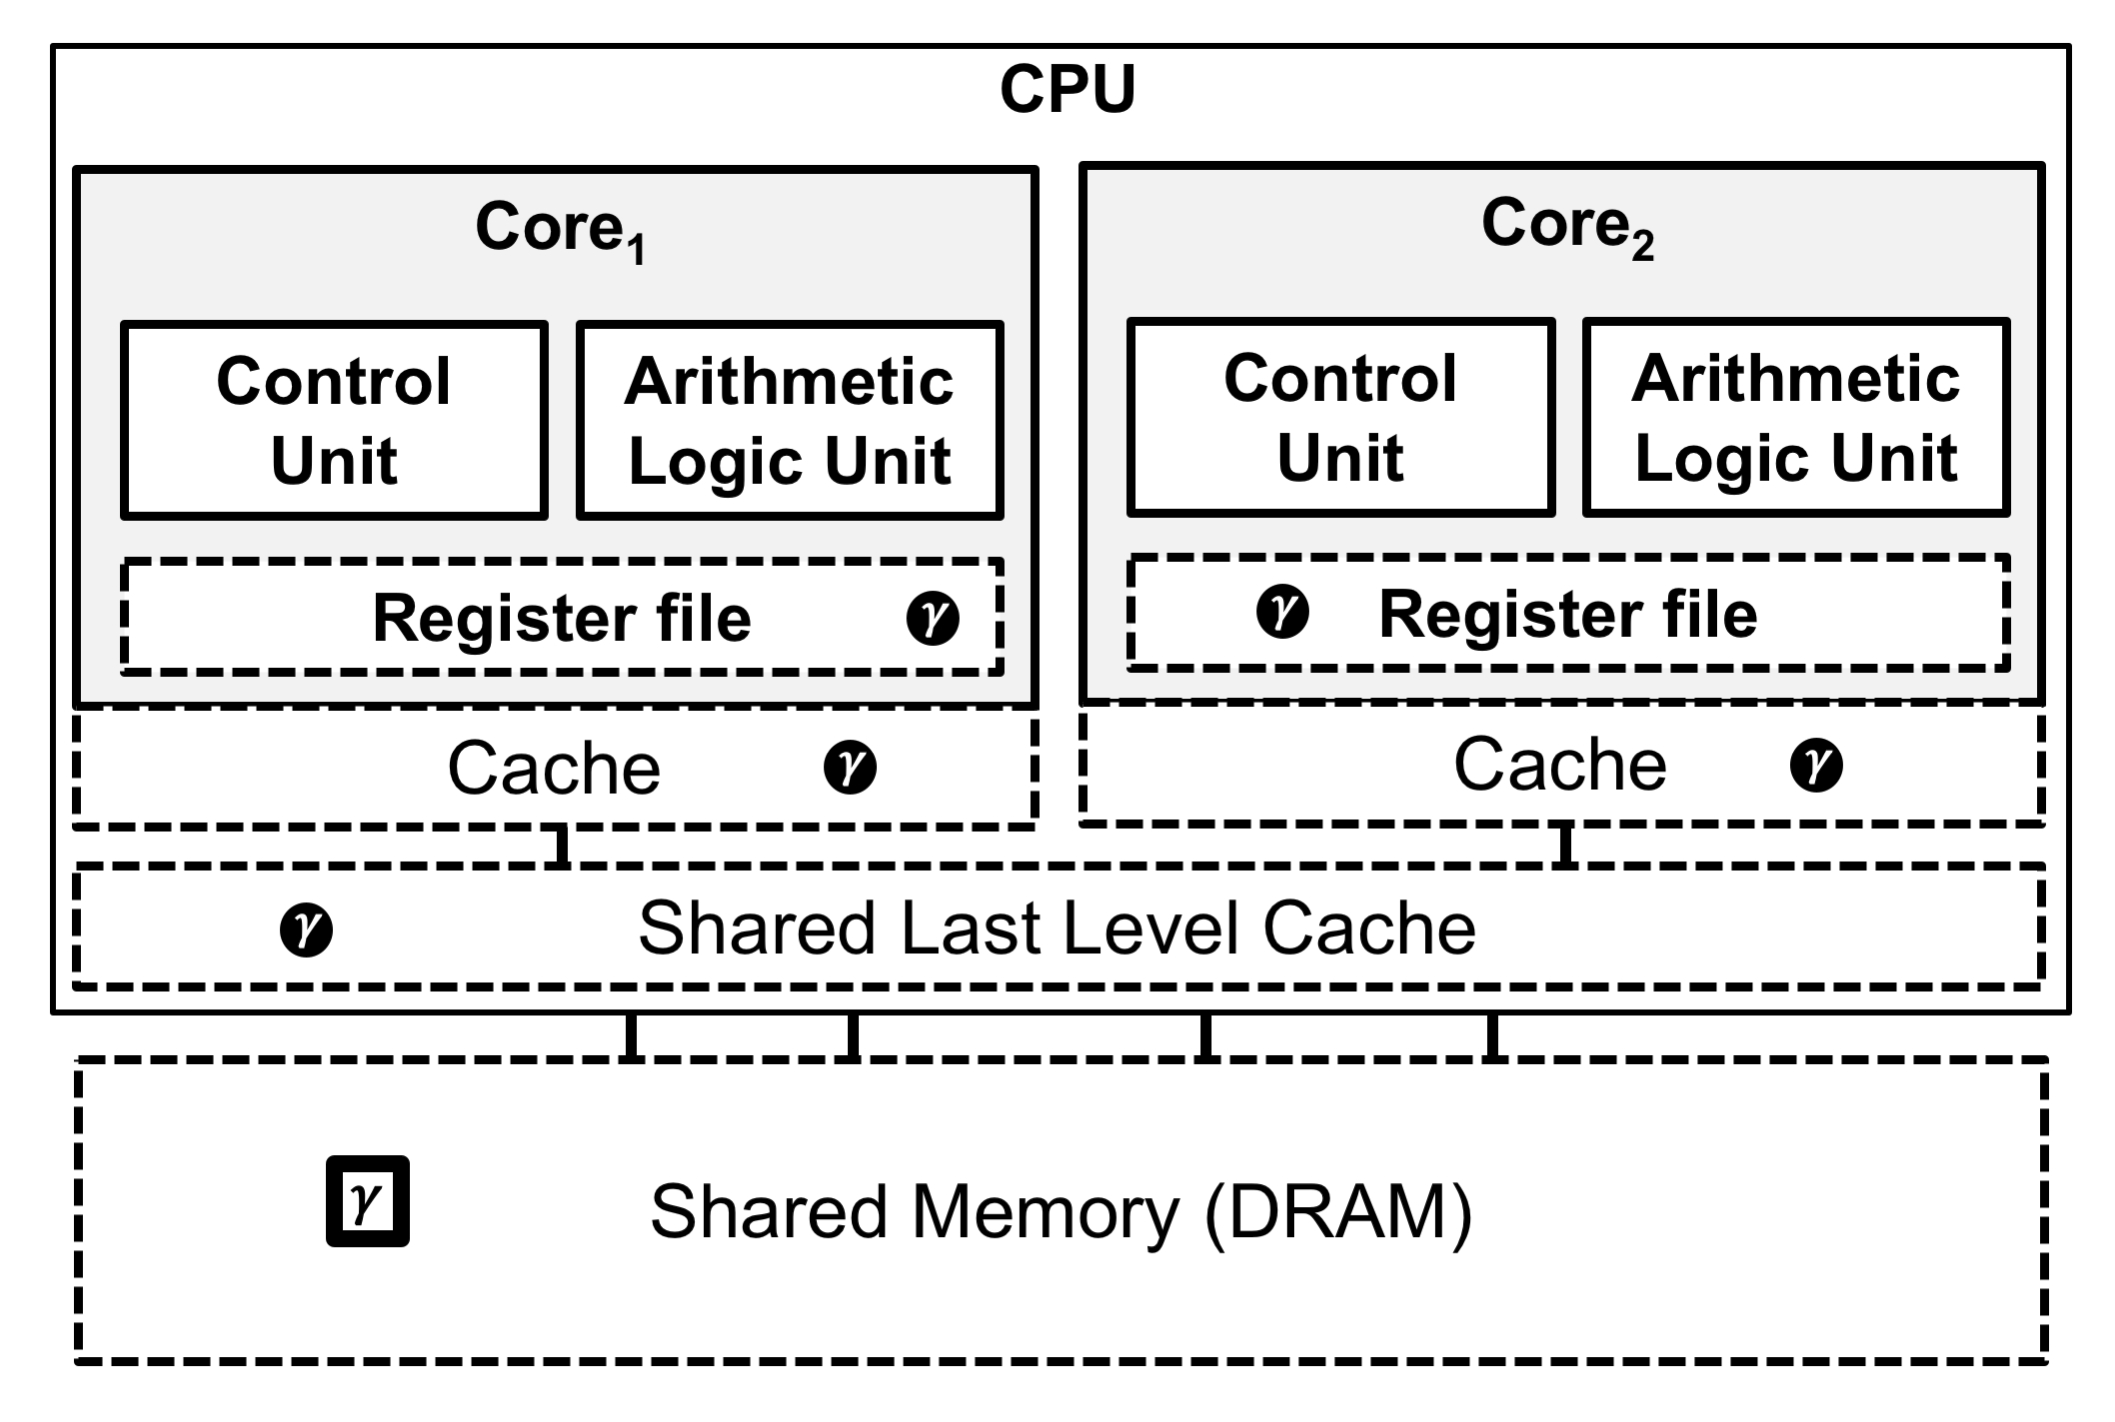
\includegraphics[width=4.5in]{\ArtDir/MemoryModel}
\centering
\caption
{\textbf{A simplified view of a dual-core CPU with the memory hierarchy highlighted through use of dashed boxes} -- \small  
A variable $\gamma$ represents a specific address in the shared memory and is shown here as a square box.  
At any given time, the value associated with this address may exist at each level in the memory as shown 
by the variable name in a black circle.
}
\label{fig:MemoryModel}
\end{figure}

Consider a variable $\gamma$ in Figure~\ref{fig:MemoryModel}.  There is only one address in the 
memory and a single value represented by the bytes at that address.  Throughout the memory hierarchy, from the
register file on down through the various levels of cache, there are temporary values for the variable $\gamma$.
A cache coherence\index{cache!coherence}\index{memory!coherence} protocol manages these values and assures 
that over time they provide a common view
of memory.  At any given moment, however, the values for $\gamma$ may be inconsistent.  In other words,
the value sitting in a register may be different than the value in the various levels of cache which may be different
from the value in DRAM.  The topic 
of \emph{memory consistency}\index{memory!consistency} addresses
these values and how they vary with respect to each other at a fixed point in time.  When they are allowed
to differ at any given point in time, we say that the system 
has a \emph{relaxed memory consistency model}\index{relaxed memory consistency}\index{memory!relaxed consistency}.



%end of: Text and table from common core book: 3


%------------------------------------------------------------------------------------------------------------------        
\section{The fundamental design patterns of OpenMP}
\label{sec:OMPpatterns}

I need a figure for the trapezoid integration for pi.

Then I'll list the three patterns we'll cover and the program we'll use to explore them.  
Take a look at figure~\ref{code:PiSeq}.  It's really pretty.  This is the serial or sequential code for the pi
program. 



\begin{itemize}
\item design patterns: SPMD, loop-level parallelism, divide-and-conquer
\end{itemize}


%Text and table from common core book: 4
\begin{figure}[!htbp]
%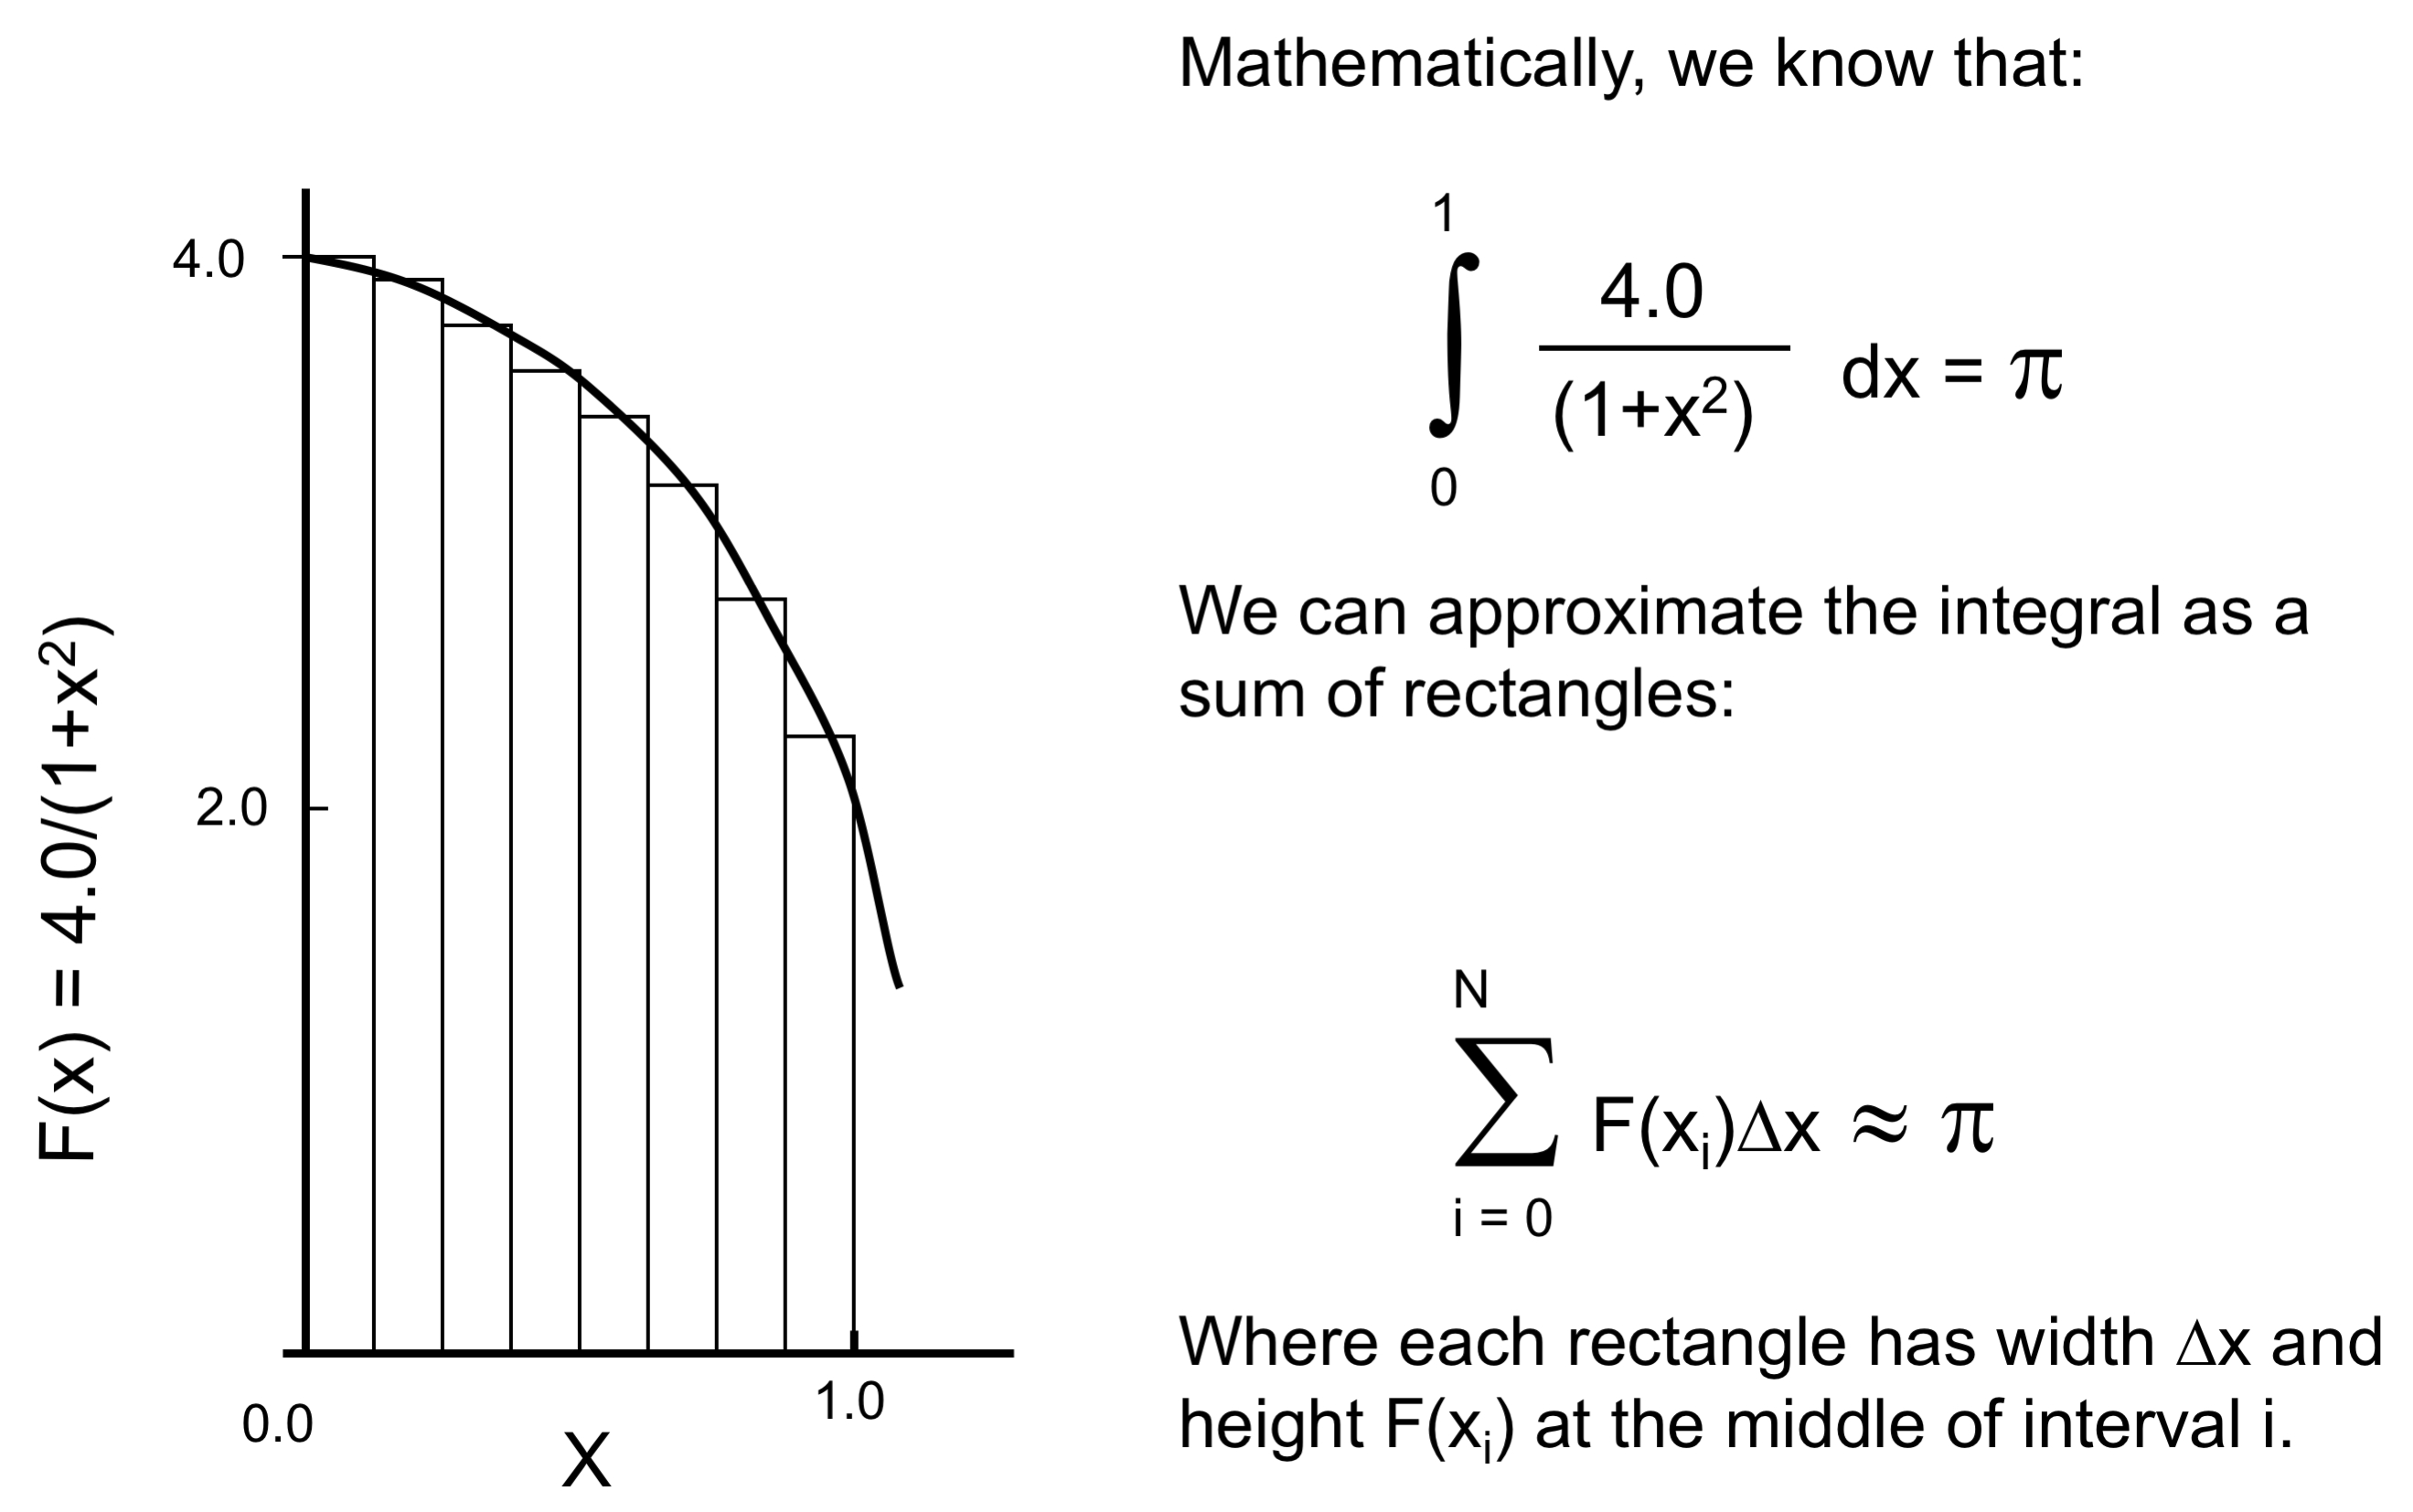
\includegraphics[width=\textwidth]{\ArtDir/pimath}
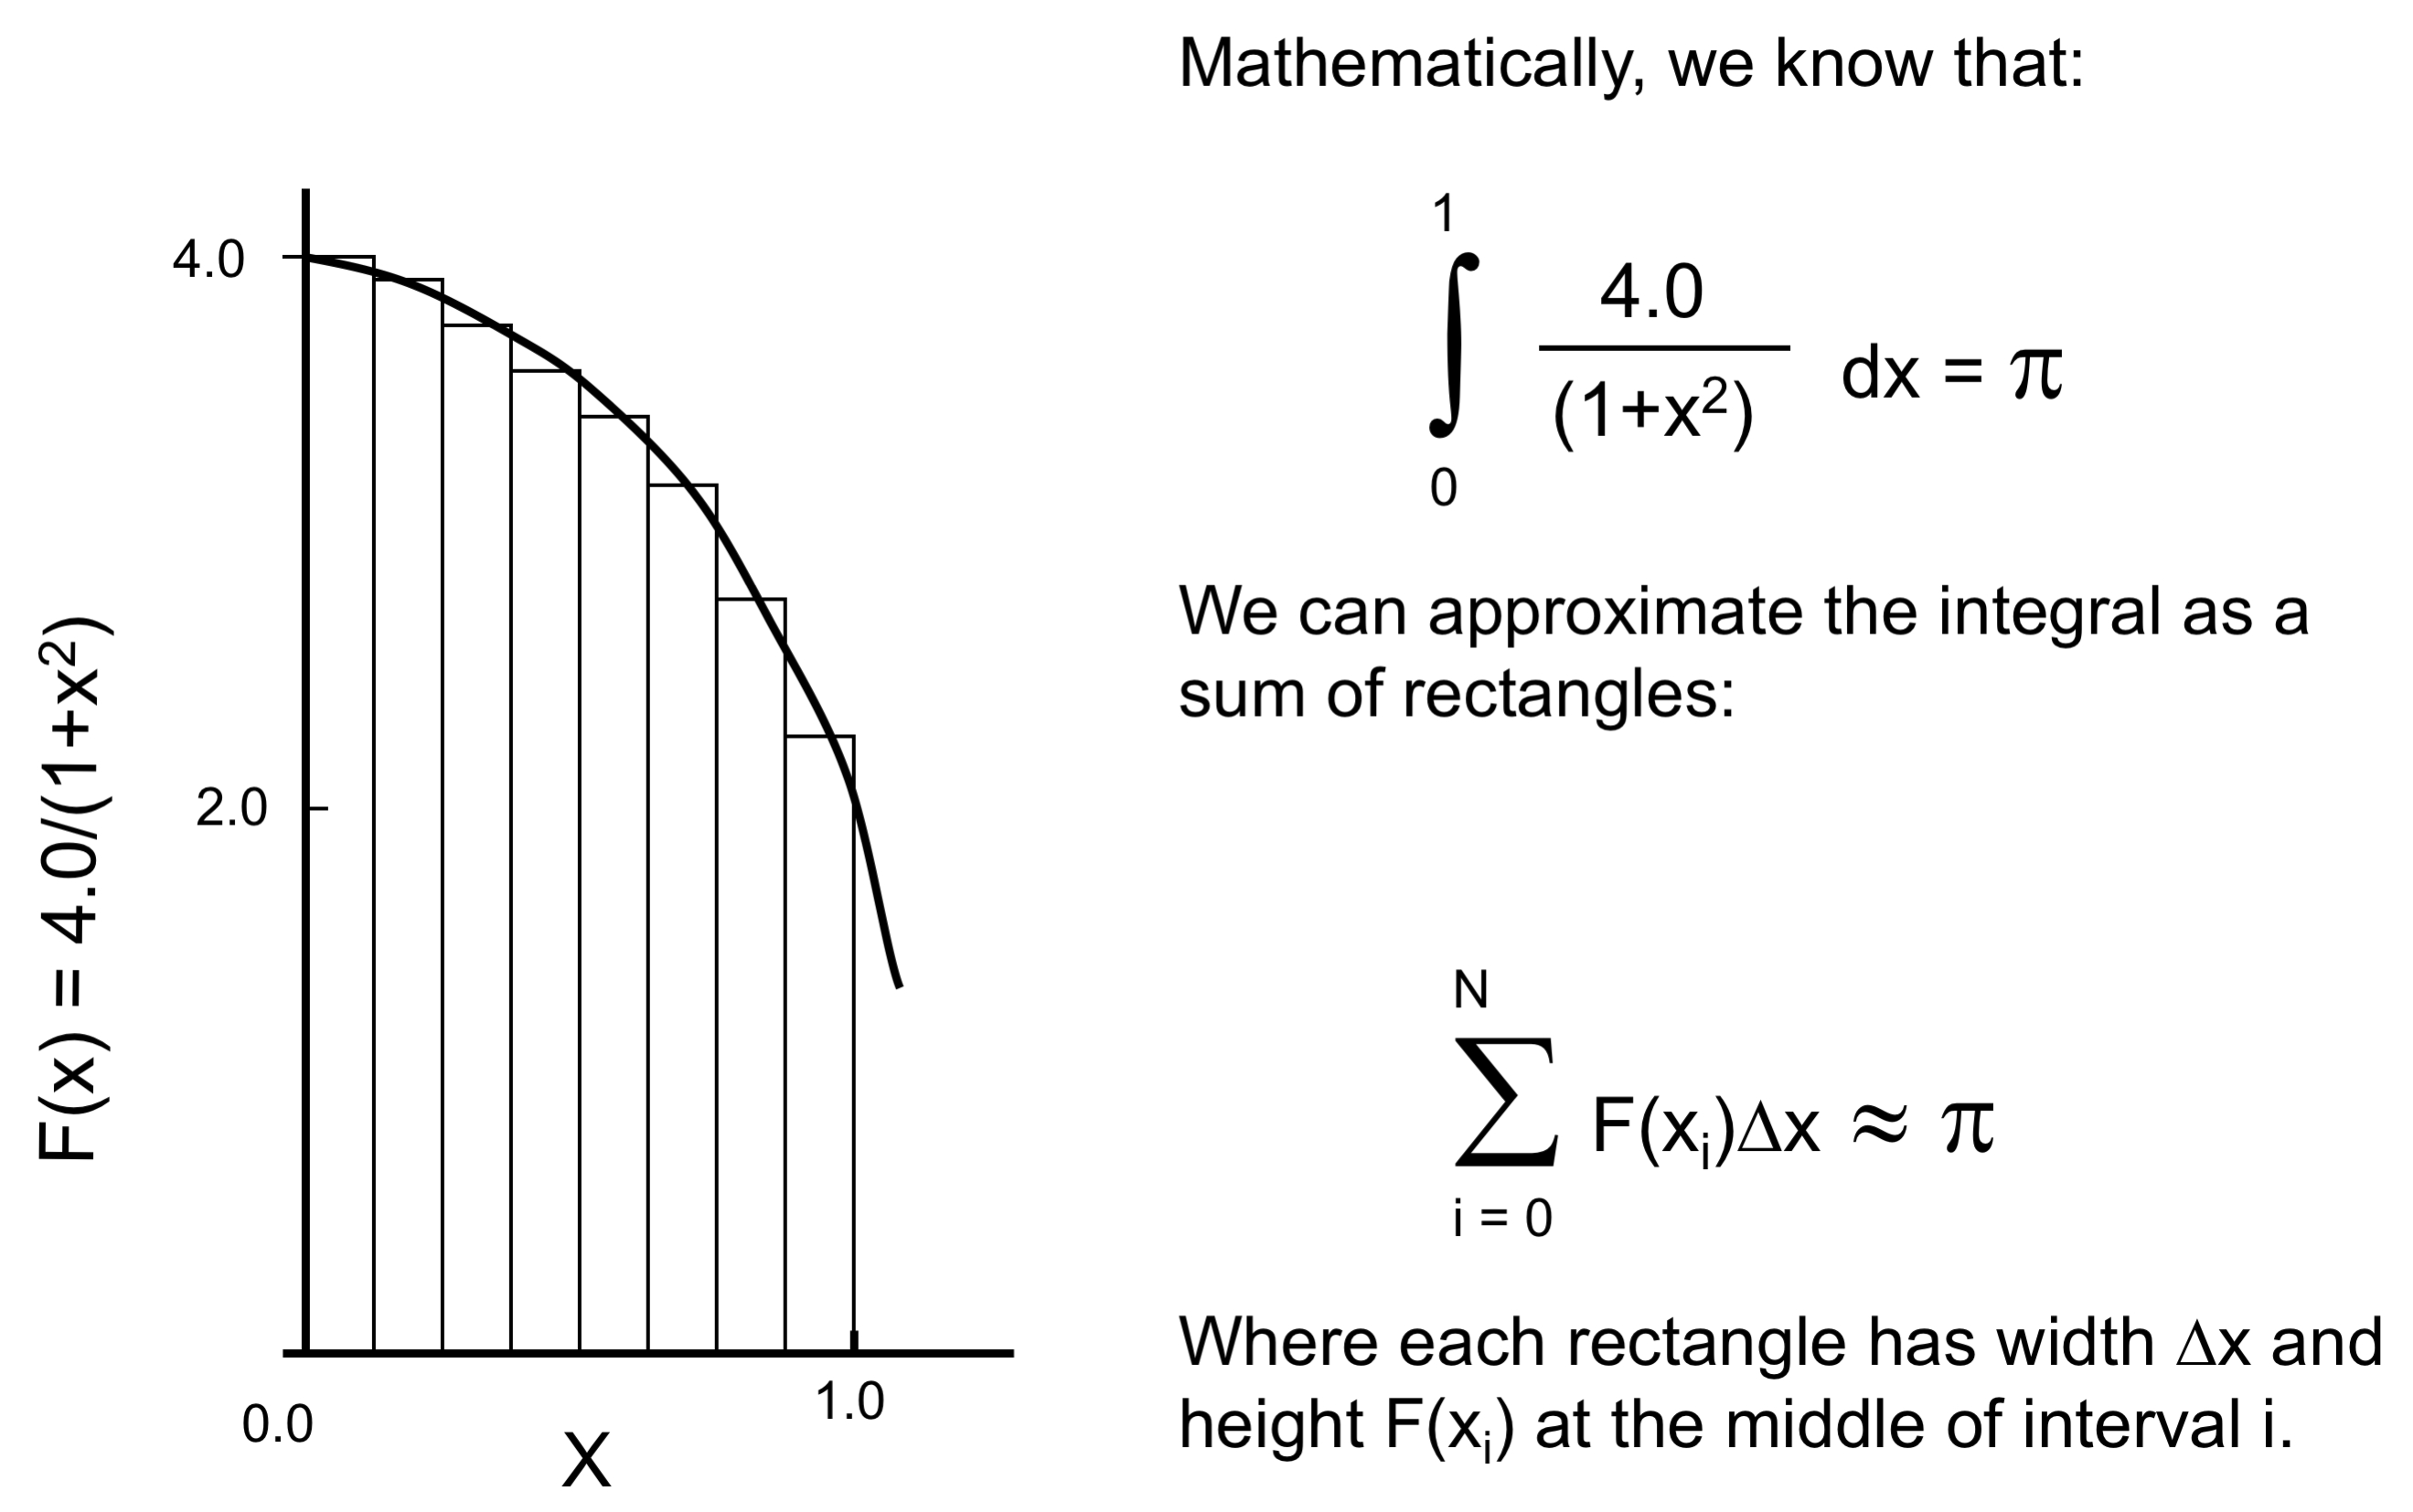
\includegraphics[width=4.2in]{\ArtDir/pimath}
\centering
\caption
{\textbf{Numerical integration} -- \small 
An integral can be approximated by filling in 
the area under a curve with rectangles and summing their areas.  We choose
the integrand and the limits of integration so the result should approximate Pi.\index{numerical integration}
}
\label{pimath}
\end{figure}
%end of: Text and table from common core book: 4




\begin{CodeExample}%
{\textbf{Sequential $\pi$ program} --\small This program carries out a numerical integration 
of a definite integral selected such that the result should be the number $\pi$.
}%
{code:PiSeq}
\begin{lstlisting}

#include <stdio.h>
#include <omp.h>
static long num_steps = 1024*1024*1024;

int main()
{
   double x, pi, step, sum = 0.0;
   step = 1.0 / (double) num_steps;

   for (int i = 0; i < num_steps; i++) {
      x = (i + 0.5) * step;
      sum += 4.0 / (1.0 + x * x);
   }

   pi = step * sum;
   printf("pi = %lf, with %ld steps\n ", pi, num_steps);
}
\end{lstlisting}
\end{CodeExample}


%------------------------------------------------------------------------------------------------------------------        
\subsection{The SPMD pattern}
\label{sec:patternsSPMD}

Memory consistency, flushes, barriers, nowait.

 
\begin{itemize}
\item Memory: stack vs heap
\item a memory consistency model and synchronization
\item default rules of data sharing
\end{itemize}




I have an SPMD parallel version of this code in figure~\ref{code:piSPMD}.
 

 
\begin{CodeExample}%
{\textbf{OpenMP $\pi$ program, SPMD pattern} --\small This program carries out a numerical integration 
of a definite integral selected such that the result should be the number $\pi$.  This code uses the 
SPMD pattern.
}%
{code:PiSPMD}
\begin{lstlisting}
#include <stdio.h>
#include <omp.h>

static long num_steps = 1024*1024*1024;
int main ()
{
   int numthreads;
   double pi, step, full_sum = 0.0;
   step = 1.0 / (double) num_steps;

   #pragma omp parallel 
   {
      int id = omp_get_thread_num();
      double x, partial_sum = 0;

      #pragma omp single
         numthreads = omp_get_num_threads();

      for (int i = id; i < num_steps; i += numthreads) {
         x = (i + 0.5) * step;
         partial_sum += 4.0 / (1.0 + x*x);
      }
      #pragma omp critical
         full_sum += partial_sum;
    }
      
   pi = step * full_sum;
   printf("\n pi is %f with %d with threads \n ", pi, numthreads);
}	  

\end{lstlisting}
\end{CodeExample}


%------------------------------------------------------------------------------------------------------------------        
\subsection{The Loop Level pattern}
\label{sec:patternsLoops}

Most programmers think of OpenMP as a system for turning serial loops into parallel loops.  Start with a well tested serial program.  
Then go through the following steps loop by loop to create a parallel program.
\begin{itemize}
\item Find a compute intensive loop.
\item Find the concurrency in the loop.  
\item Transform the loop body to expose the concurrency; that is, make changed needed 
so the loop iterations can execute in any order and the result will still be correct.
\item Add OpenMP directives to run the concurrent iterations in parallel
\end{itemize}
We show and example of this process in figure-pi-program



\begin{itemize}
  \item Worksharing loops: parallel for.
  \item Clauses to change effects: num\_threads, etc.
  \item schedule(static) important to introduce as will need it later.
  \item collapse() clause.
\end{itemize}

\begin{itemize}
\item The openMP data environment clauses: private, firstprivate, shared.  default(none) clauses
\item Do we need threadprivate?  No, we do not.
\item worksharing loops including collapse, reduction, and schedule clauses
\item for the schedule clauses, only cover static. 
\end{itemize}


\begin{CodeExample}%
{\textbf{Parallel $\pi$ program, Loop parallelism pattern} --\small This program carries out a numerical integration 
of a definite integral selected such that the result should be the number $\pi$.
}%
{code:PiLoop}
\begin{lstlisting}

#include <stdio.h>
#include <omp.h>
static long num_steps = 100000000;

int main ()
{
   double x, pi, step, sum = 0.0;
   int numthreads;
   step = 1.0 / (double) num_steps;

    #pragma omp parallel  
    {
         #pragma omp single
              numthreads =omp_get_num_threads();

         #pragma omp for private(x) reduction(+:sum) 
            for (int i = 0; i < num_steps; i++){
                 x = (i + 0.5) * step;
                 sum = sum + 4.0 / (1.0 + x*x);
	     }
     }
    pi = step * sum;
    printf("\n pi is %f with %d threads\n", pi,numthreads);
}	  
\end{lstlisting}
\end{CodeExample}


%------------------------------------------------------------------------------------------------------------------        
\subsection{The Divide and Conquer pattern}
\label{sec:patternsDivCon}

\begin{itemize}
\item The openMP data environment (task specific): private, firstprivate, shared.  
\item explicit tasks and how tasks interact with the data environment.
\item when do tasks complete and taskwait
\item Asynchrony with tasks (task with nowait)
\end{itemize}


%Text and table from common core book: 5

With the divide and conquer pattern, we recursively split the problem into smaller and smaller sub-problems,
continuing until the sub-problems become so small that it makes sense to just solve them directly.
Then we reverse the process taking our directly solved sub-solutions and merging them up the tree
to generate the final solution. 
Figure~\ref{fig:divide_conquer} illustrates this divide and conquer pattern.   

\begin{figure}[!htbp]
\centering
%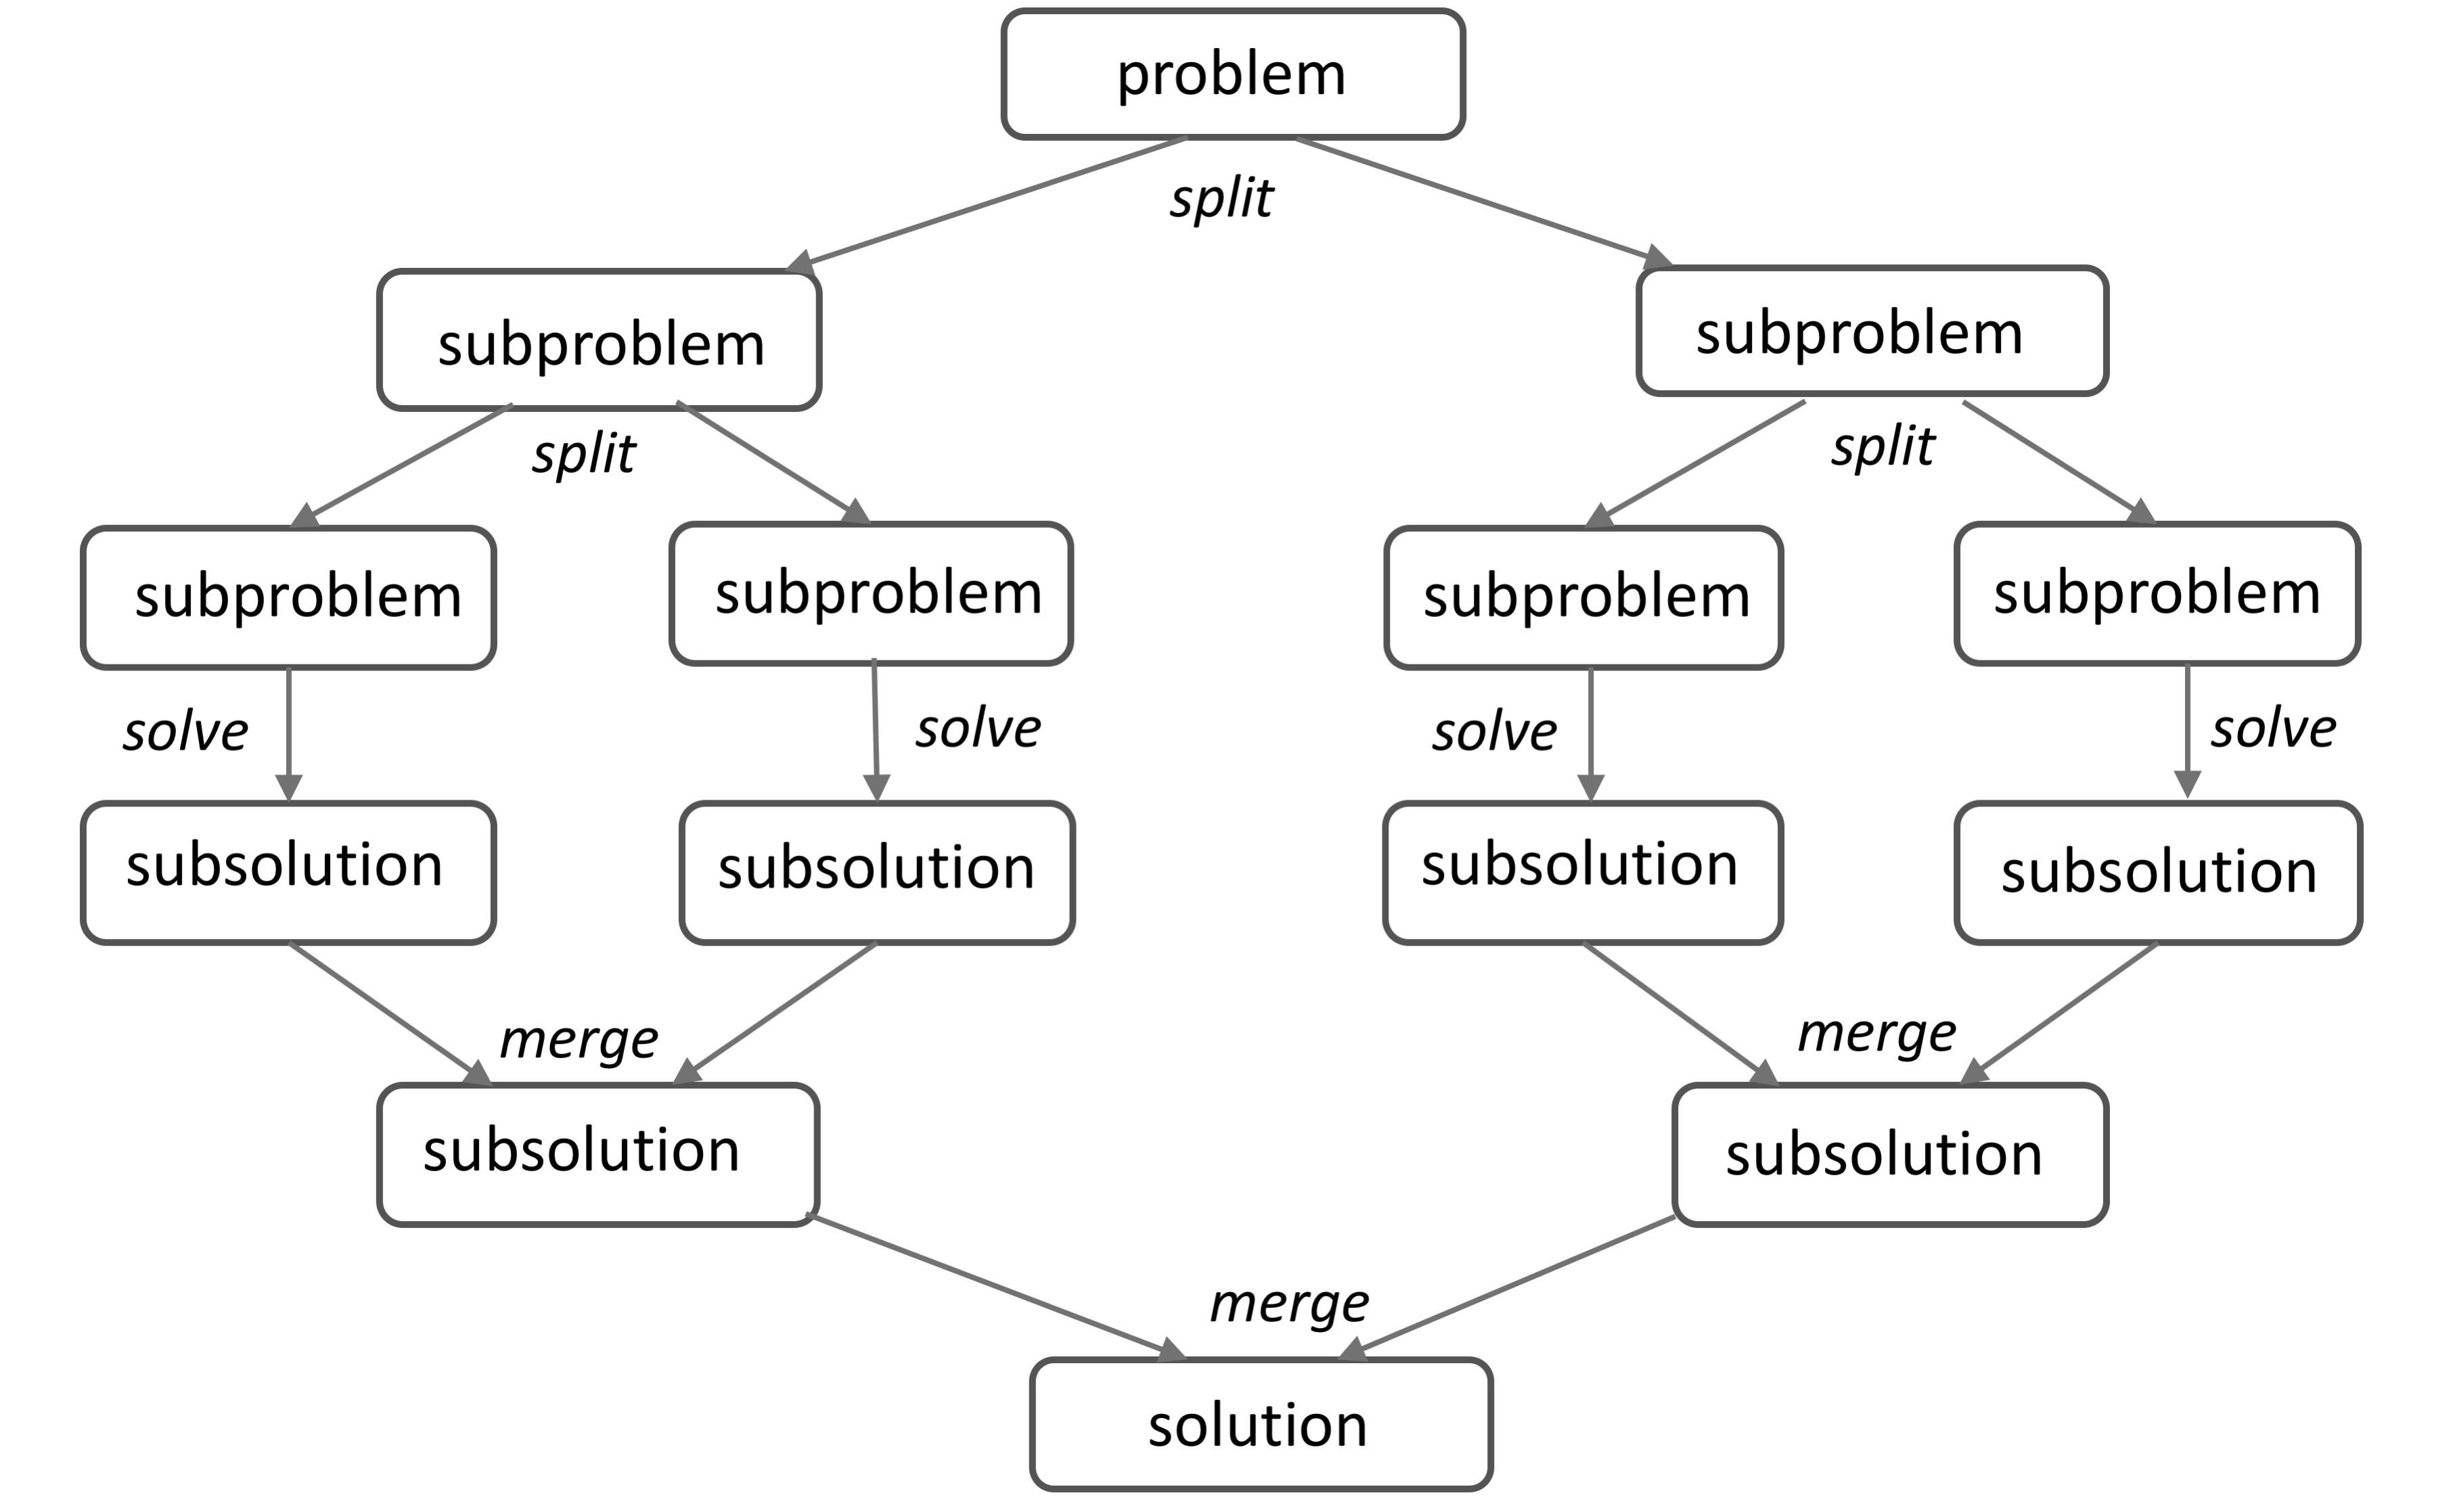
\includegraphics[width=\textwidth]{\ArtDir/DivideConquer}
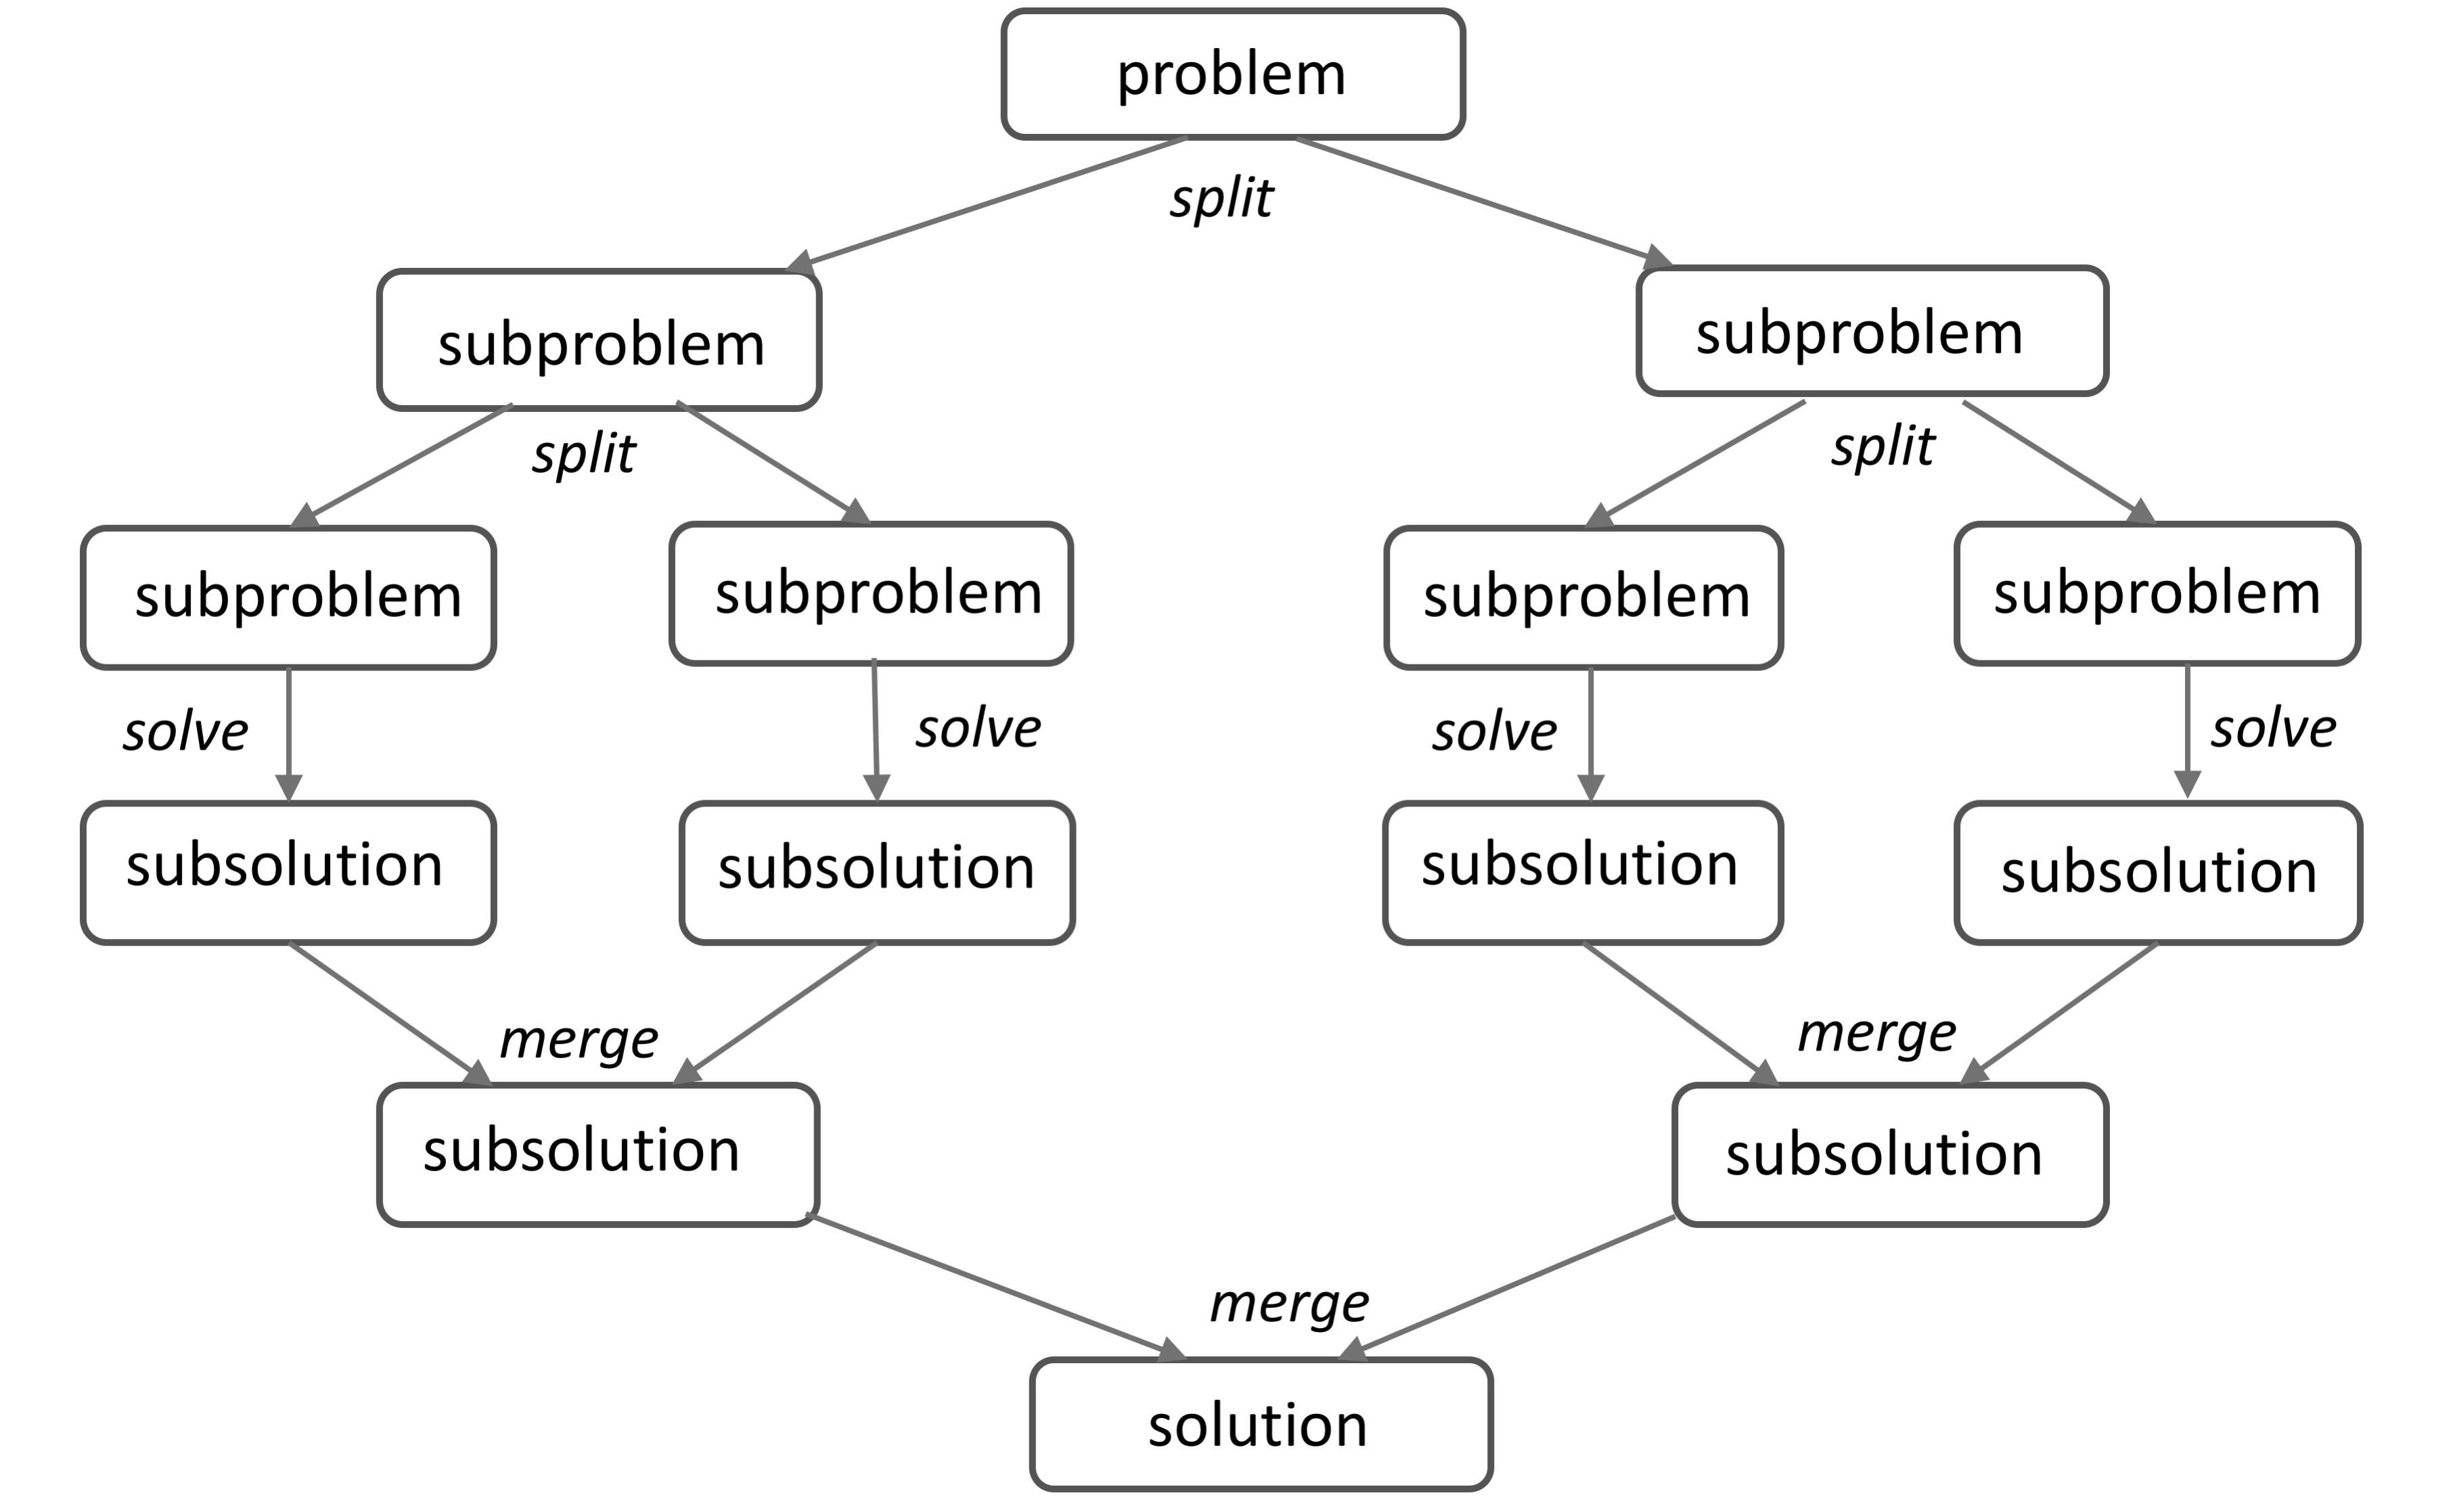
\includegraphics[width=4.6in]{\ArtDir/DivideConquer}
\centering
\caption
{\textbf{Illustration of the divide and conquer pattern} -- \small
The pattern breaks down
into three parts: a recursive splitting into a tree of subproblems, a direct solve, and 
then merging ``back up the tree'' to obtain the overall solution.
} 
\label{fig:divide_conquer}
\end{figure}

One of the decisions to make when implementing a divide and conquer algorithm is 
when to do the direct solve.
In our Fibonacci program, we split all the way down to \code{fib(1)} and \code{fib(2)}.
Usually, you define the base case (i.e., the size problem where you solve directly) to be
much larger, to balance the cost of splitting into smaller and smaller subproblems compared to 
the cost of a direct solve.  For example, in a divide and conquer linear equation solver, you might
choose the base case to be the size of the problem that just fills the last level cache of your processor.  

In general with this pattern, there are 3 options for doing work: you can do it as you split into sub-problems, or
you can do work only at the leaves (at the solve step), or you can 
do work as you recombine (as you merge sub-solutions).   Parallelism emerges naturally from this pattern as each 
of the individual solve, split, and merge steps can usually proceed in parallel.   





%end of: Text and table from common core book: 5


While we are at it, we have figure~\ref{code:PiLoop} figure~\ref{code:PiSeqDivCon} figure~\ref{code:PiParDivCon}


\begin{CodeExample}%
{\textbf{Sequential $\pi$ program, divide and conquer} --\small This program carries out a numerical integration 
of a definite integral selected such that the result should be the number $\pi$.
}%
{code:PiSeqDivCon}
\begin{lstlisting}

#include <omp.h>
#include <stdio.h>
static long num_steps = 1024*1024*1024;
#define MIN_BLK 1024*256
double pi_comp(int Nstart, int Nfinish, double step)
{   
   int iblk;
   double x, sum = 0.0, sum1, sum2;
   if (Nfinish - Nstart < MIN_BLK){
      for (int i = Nstart; i < Nfinish; i++) {
         x = (i + 0.5) * step;
         sum += 4.0 / (1.0 + x * x);
      }
   }
   else {
      iblk = Nfinish - Nstart;
      sum1 = pi_comp(Nstart, Nfinish - iblk/2, step);
      sum2 = pi_comp(Nfinish - iblk/2, Nfinish, step);
      sum = sum1 + sum2;
   }
   return sum;
}

int main () 
{
   int i;
   double step, pi, sum;
   step = 1.0 / (double) num_steps;

   sum = pi_comp(0, num_steps, step);
   pi = step * sum;

   printf(" for %ld steps pi = %f \n", num_steps, pi);
} 
\end{lstlisting}
\end{CodeExample}

\begin{CodeExample}%
{\textbf{Parallel $\pi$ program, divide and conquer with tasks} --\small This program carries out a numerical integration 
of a definite integral selected such that the result should be the number $\pi$.
}%
{code:PiParDivCon}
\begin{lstlisting}

#include <omp.h>
#include <stdio.h>
static long num_steps = 1024*1024*1024;
#define MIN_BLK 1024*256

double pi_comp(int Nstart,int Nfinish,double step)
{ 
   int iblk;
   double x, sum = 0.0, sum1, sum2;
   if (Nfinish - Nstart < MIN_BLK) {
      for (int i = Nstart; i < Nfinish; i++){
         x = (i + 0.5) * step;
         sum = sum + 4.0 / (1.0 + x*x); 
      }
   }
   else {
      iblk = Nfinish - Nstart;
      #pragma omp task shared(sum1)
         sum1 = pi_comp(Nstart, Nfinish - iblk/2, step);
      #pragma omp task shared(sum2)
         sum2 = pi_comp(Nfinish - iblk/2, Nfinish, step);
      #pragma omp taskwait
         sum = sum1 + sum2;
   }
   return sum;
}

int main ()
{
   double step, pi, sum;
   step = 1.0 / (double) num_steps;

      #pragma omp parallel 
      {
         #pragma omp single
         {
            printf("num threads=%d", omp_get_num_threads());
            sum = pi_comp(0, num_steps, step);
         }
      }
      pi = step * sum;
      printf(" for %ld steps pi = %f \n", num_steps, pi);
}  
\end{lstlisting}
\end{CodeExample}

%------------------------------------------------------------------------------------------------------------------        
\section{Tasks and the nature of OpenMP's execution model}
\label{sec:TasksExecModel}

\begin{itemize}
\item The concept of a task
\item Definition of data environments in terms of tasks ... implied vs explicit tasks.
\item tied tasks, untied tasks, and nowait
\item we need mergeable tasks since ``A target task is mergable and untied''.
\item tasks and their role in understanding the core of OpenMP.  Initial tasks and implicit tasks
\item explicit tasks and how tasks interact with the data environment.
\end{itemize}

%------------------------------------------------------------------------------------------------------------------        
\section{Our journey ahead}
\label{sec:OMPJouney}

Show the pragmas (BUD) needed to run a parallel program on a GPU.
This sets out the climax of the book, and excites that this book is going to explain it.


Introduce Matrix Multiply and
\Code{#pragma target teams distribute parallel for simd collapse(2)}
NB: put the arrays on the stack.


\begin{CodeExample}%
{\textbf{Matrix Multiplication program} --\small This program will multiply two matrices $A$ and $B$
to produce a third $C$ which has been set to zero, running on the target device.
All arrays have been previously allocated in stack memory.
}%
{code:matmulTarget}
\begin{lstlisting}
void matmul(int Ndim, int Mdim, int Pdim,
            float A[Ndim][Pdim], float B[Pdim][Mdim], float C[Ndim][Mdim]) {

  #pragma omp target teams distribute parallel for simd collapse(2)
  for (int i = 0; i < Ndim; i++) {
    for (int j = 0; j < Mdim; j++) {
      for(int k = 0; k < Pdim; k++) {
	C[i][j] += A[i][k] * B[k][i];
      }
    }
  }
}
\end{lstlisting}
\end{CodeExample}
